\documentclass[mathserif,hyperref={urlcolor=cyan,colorlinks=true}]{beamer}
\usepackage[utf8]{inputenc}

\usetheme{Warsaw}

\usepackage[T1]{fontenc}
\usepackage{multicol}

\usepackage{minted}
\usemintedstyle{monokai}

\newminted{bash}{fontsize=\fontsize{7}{7}}
\newminted{c}{fontsize=\fontsize{7}{7}}
\newminted{diff}{fontsize=\fontsize{7}{7}}
\newminted{perl}{fontsize=\fontsize{7}{7}}
\newminted{console}{fontsize=\fontsize{7}{7}}
\definecolor{bgc}{HTML}{272822}

\beamertemplatenavigationsymbolsempty
\setbeamertemplate{headline}{}
\setbeamertemplate{footline}{}

\title{On The Importance Of Rabbits}
\author{Sergey Aleynikov}
\date[August 2017]{YAPC::EU 2017}

\begin{document}{

\begin{frame}
\titlepage
\end{frame}

\begin{frame}
\center{
\scalebox{0.3}{
    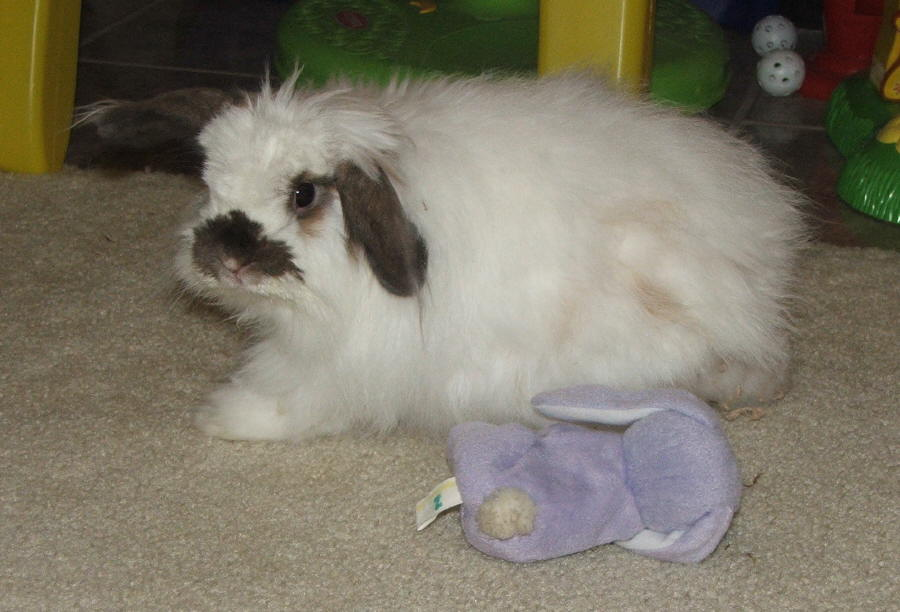
\includegraphics{lop.jpg}
}
}
\end{frame}


\begin{frame}
\center{
\scalebox{0.25}{
    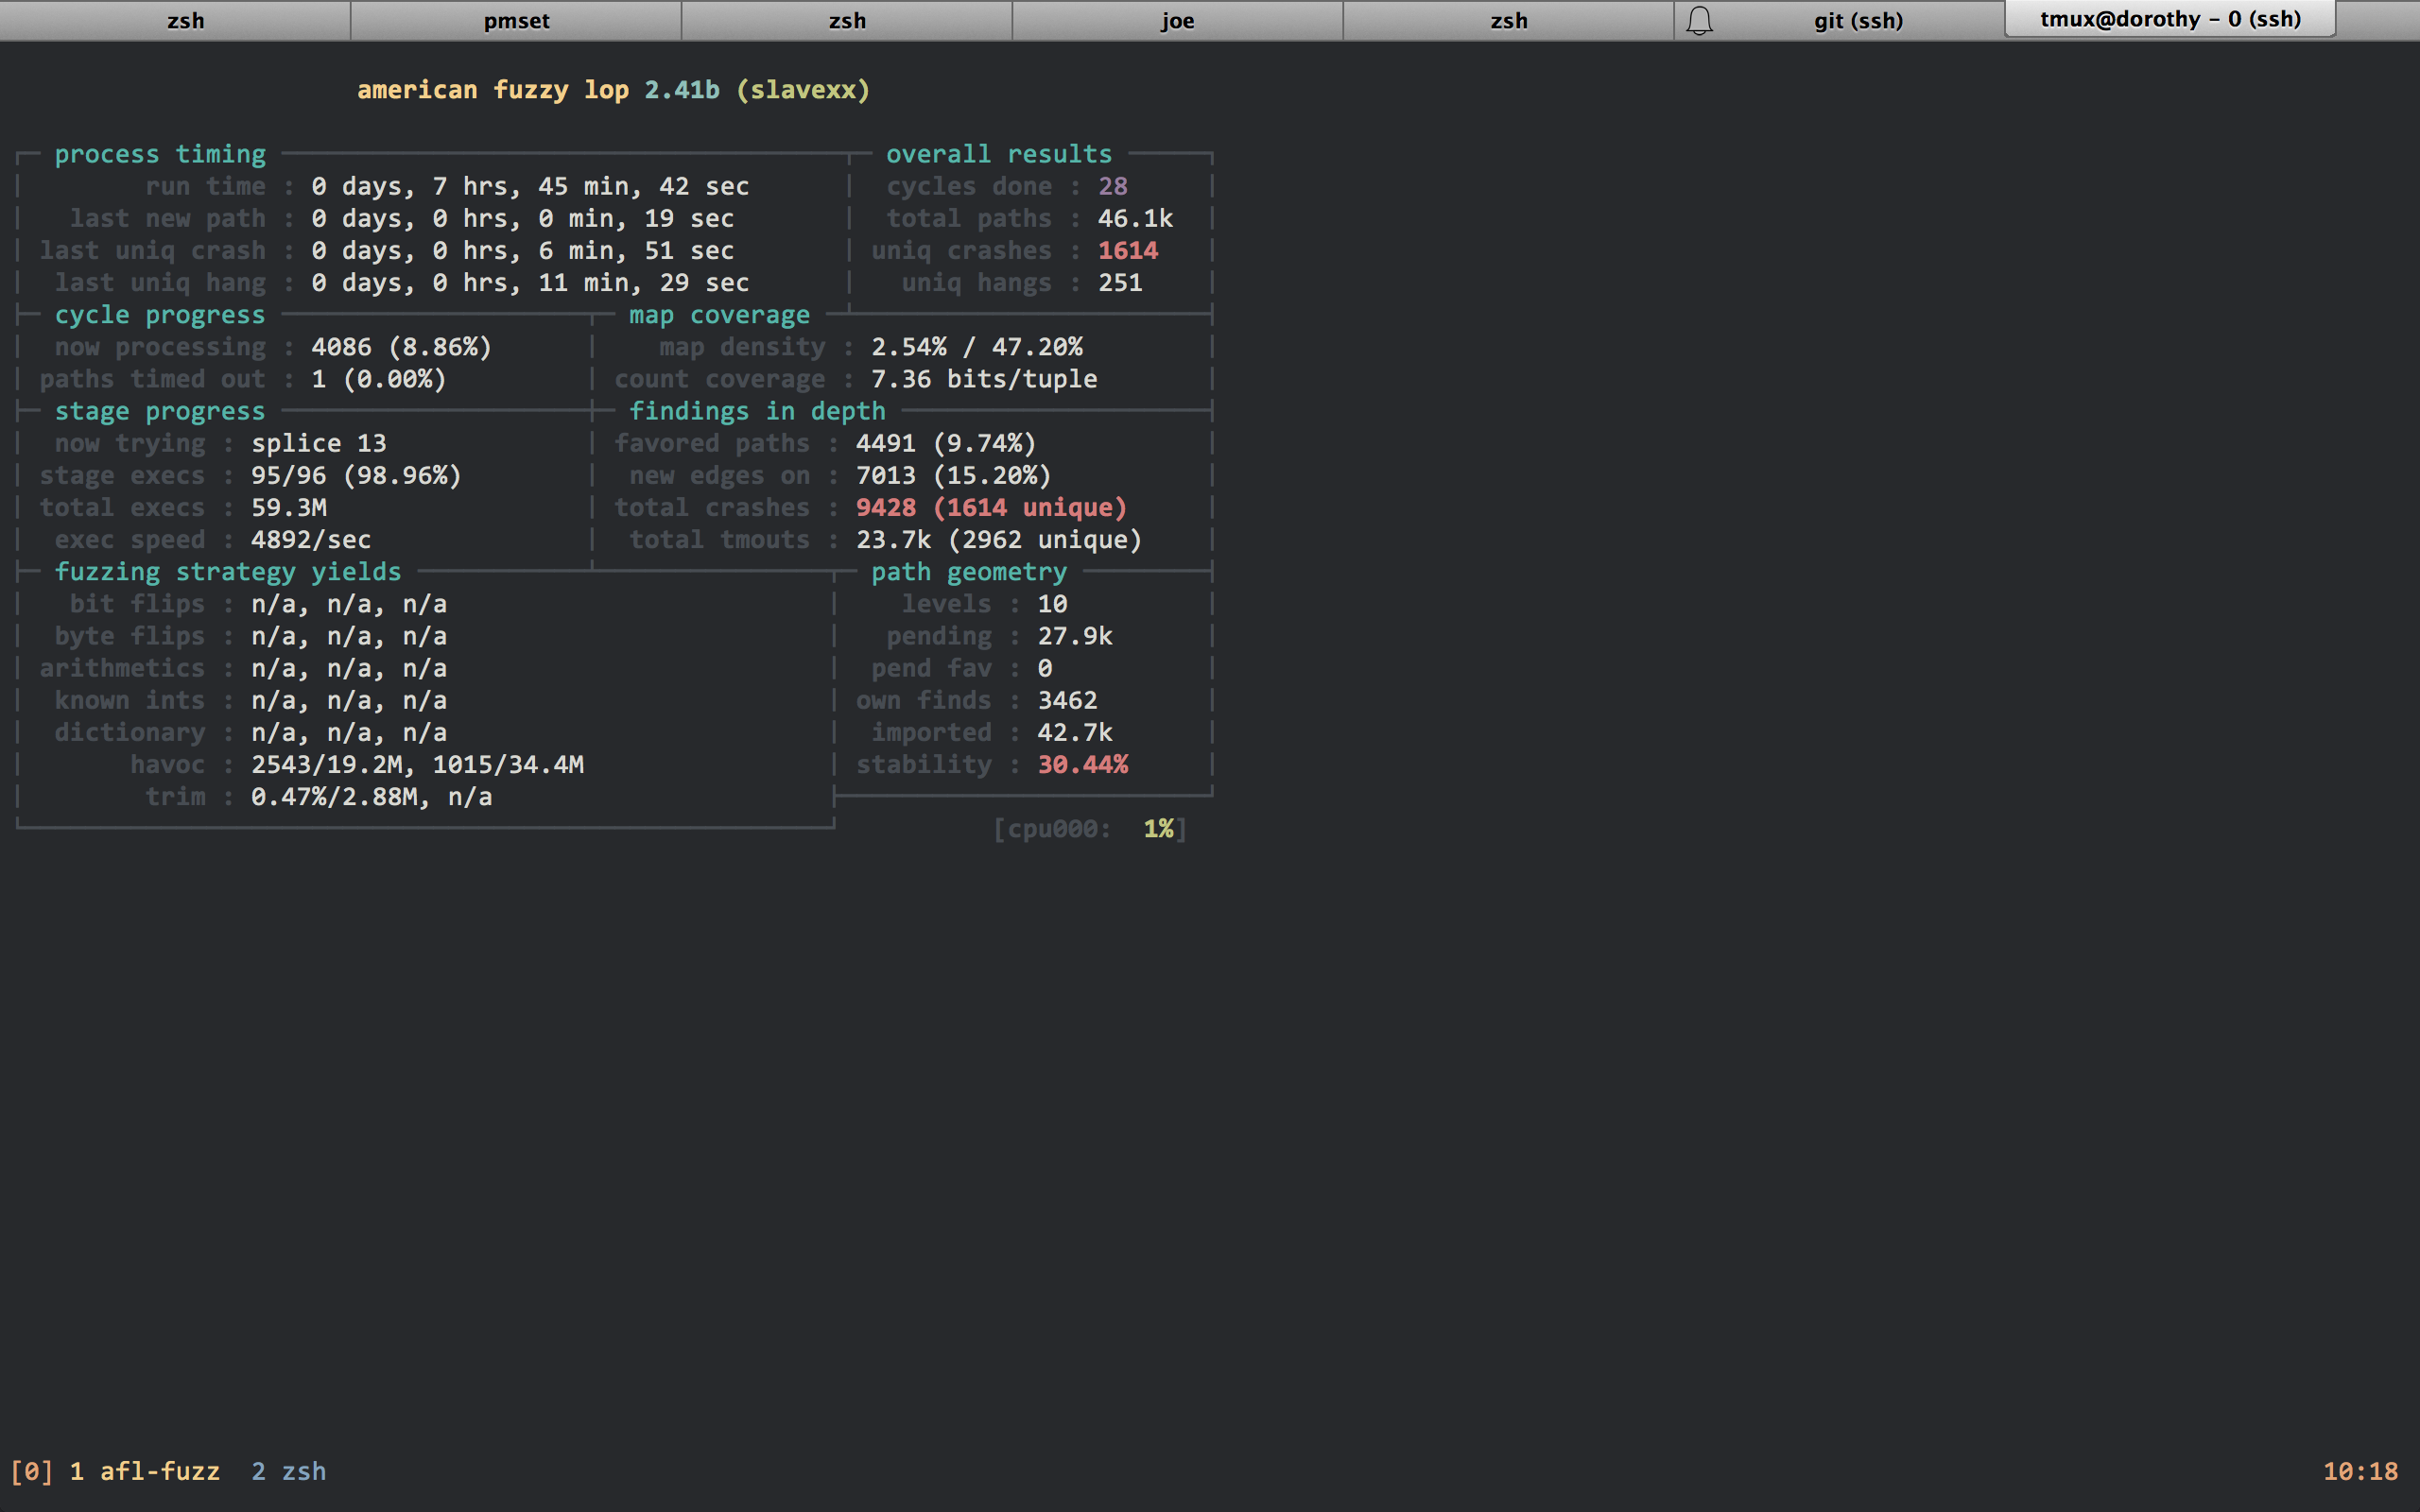
\includegraphics{main.png}
}
}
\end{frame}

{
\color{white}
\setbeamercolor{background canvas}{bg=bgc}
\setbeamercolor{item}{fg=white}
\setbeamercolor{itemize/enumerate body}{fg=white}

\begin{frame}[fragile]
\begin{bashcode}
./Configure -des -Dusedevel -DDEBUGGING -Dcc=afl-clang-fast
AFL_HARDEN=1 make -j20 test_prep

\end{bashcode}
\pause
\begin{bashcode}

AFL_PRELOAD=/usr/local/lib/afl/libdislocator.so \
afl-fuzz -x keywords -o afl-out -i indir -t 80 -m 350 \
./perl @@
\end{bashcode}
\end{frame}

\begin{frame}[fragile]
\begin{diffcode}
diff --git a/config.h b/config.h
index 58f56c8..43ae4ee 100644

-#define MAX_DET_EXTRAS      200
+#define MAX_DET_EXTRAS      500

-#define MAX_AUTO_EXTRAS     (USE_AUTO_EXTRAS * 10)
+#define MAX_AUTO_EXTRAS     (USE_AUTO_EXTRAS * 30)

-#define MAP_SIZE_POW2       16
+#define MAP_SIZE_POW2       17
\end{diffcode}
\end{frame}

\begin{frame}
\center{
\huge
BANG!
}\end{frame}

\begin{frame}
\begin{itemize}
\item fork()ed proccesses
\item symlink()ed files
\item unlink()ed files
\pause
\item ... and so on
\end{itemize}
\end{frame}


\begin{frame}[fragile]
\begin{ccode}
STATIC OP*
push_one() {
    dSP; dTARGET;

    XPUSHi(42);
    PUTBACK;

    return NORMAL;
}

PL_ppaddr[OP_FORK] = push_one;
\end{ccode}

\pause

\begin{ccode}
STATIC OP*
fake_backtick() {
    dSP; dTARGET;
    const U8 gimme = GIMME_V;
    POPs;

    if (gimme != G_VOID) {
        XPUSHi(42);
        PUTBACK;
    }

    return NORMAL;
}

PL_ppaddr[OP_BACKTICK] = fake_backtick;

\end{ccode}
\end{frame}


\begin{frame}[fragile]
\begin{perlcode}
    PL_ppaddr[OP_FORK] = push_one;
    PL_ppaddr[OP_BACKTICK] = fake_backtick;
    PL_ppaddr[OP_DUMP] = pop_none;
    PL_ppaddr[OP_EXIT] = push_noarg;
    PL_ppaddr[OP_RAND] = push_noarg;
    PL_ppaddr[OP_SRAND] = push_noarg;
    PL_ppaddr[OP_SLEEP] = push_noarg;
    #PL_ppaddr[OP_UNPACK] = pop_pop_push;

    PL_ppaddr[OP_EXEC] = clearlist_pushone;
    PL_ppaddr[OP_SYSTEM] = clearlist_pushone;
    PL_ppaddr[OP_REQUIRE] = pop_none;
    PL_ppaddr[OP_DOFILE] = pop_none;

    PL_ppaddr[OP_UNLINK] = clearlist_pushone;
    PL_ppaddr[OP_CHROOT] = pop_none;
    PL_ppaddr[OP_CHMOD] = clearlist_pushone;
    PL_ppaddr[OP_OPEN_DIR] = pop_one;
    PL_ppaddr[OP_CHOWN] = clearlist_pushone;
    PL_ppaddr[OP_LINK] = pop_one;
    PL_ppaddr[OP_TRUNCATE] = pop_one;
    PL_ppaddr[OP_KILL] = clearlist_pushone;
    PL_ppaddr[OP_RENAME] = pop_one;
    PL_ppaddr[OP_RMDIR] = pop_none;
    PL_ppaddr[OP_ALARM] = pop_none;

    PL_ppaddr[OP_LISTEN] = pop_one;
    PL_ppaddr[OP_OPEN] = clearlist_pushone;
    PL_ppaddr[OP_READ] = clearlist_pushone;
    PL_ppaddr[OP_SYSREAD] = clearlist_pushone;
    PL_ppaddr[OP_RECV] = clearlist_pushone;
    PL_ppaddr[OP_SYSCALL] = clearlist_pushone;
    PL_ppaddr[OP_MKDIR] = pop_maybearg;
\end{perlcode}
\end{frame}



\begin{frame}[fragile]
\begin{bashcode}
% time perl -e1
perl -e1  0.00s user 0.00s system 0% cpu 0.002 total
% perl -e 'print 1/0.002'
500
\end{bashcode}
\end{frame}

\begin{frame}[fragile]
\begin{diffcode}
--- a/ext/ExtUtils-Miniperl/lib/ExtUtils/Miniperl.pm
+++ b/ext/ExtUtils-Miniperl/lib/ExtUtils/Miniperl.pm
@@ -93,6 +93,8 @@ static struct perl_vars* my_plvarsp;
 struct perl_vars* Perl_GetVarsPrivate(void) { return my_plvarsp; }
 #endif

+volatile char *__afl_persistent_sig = "##SIG_AFL_PERSISTENT##";
+
 #ifdef NO_ENV_ARRAY_IN_MAIN
 extern char **environ;
 int
@@ -153,6 +155,12 @@ main(int argc, char **argv, char **env)
        PL_perl_destruct_level = 0;
     }
     PL_exit_flags |= PERL_EXIT_DESTRUCT_END;
+
+    int foo = memcmp(__afl_persistent_sig, "abc", 3);
+    if (foo > 2) exit(0);
+
     exitstatus = perl_parse(my_perl, xs_init, argc, argv, (char **)NULL);
     if (!exitstatus)
         perl_run(my_perl);
\end{diffcode}
\end{frame}


\begin{frame}[fragile]
\begin{ccode}
extern int __afl_persistent_loop(unsigned int);

const int ITERATIONS = 1000;
const int BUFSIZE = 8 * 1024;

int len;
char buf[BUFSIZE];

while (__afl_persistent_loop(ITERATIONS) > 0) {
    bzero(buf, BUFSIZE);
    len = read(0, buf, BUFSIZE - 1024);

    ENTER;
    SAVETMPS;

    SV* sv_buf = newSVpvn_flags(buf, len, SVs_TEMP);
    eval_sv(sv_buf, G_VOID);

    FREETMPS;
    LEAVE;
}
\end{ccode}
\end{frame}

\begin{frame}[fragile]
\begin{bashcode}
AFL_PRELOAD=/usr/local/lib/afl/libdislocator.so \
afl-fuzz -x keywords -o afl-out -i indir -t 80 -m 350 \
./perl @@
\end{bashcode}
\pause
\begin{bashcode}
AFL_PRELOAD=/usr/local/lib/afl/libdislocator.so \
afl-fuzz -x keywords -o afl-out -i indir -t 80 -m 350 \
./perl
\end{bashcode}
\end{frame}


\begin{frame}[fragile]
\begin{perlcode}
use v5.24.0;
use experimental "smartmatch";
use experimental "postderef";
use experimental "refaliasing";
use experimental "regex_sets";
use experimental "signatures";
use experimental "switch";

\end{perlcode}
\pause
\begin{bashcode}

% time perl features.pl
perl features.pl   0.02s user 0.00s system 80% cpu 0.020 total
% perl -e 'print 1/0.020'
50
\end{bashcode}
\end{frame}

\begin{frame}[fragile]
\begin{perlcode}
BEGIN {
  $^H = 469895648;
  %^H = map {$_ => 1} qw/
    feature_evalbytes feature_postderef feature_refaliasing
    feature___SUB__ feature_fc feature_postderef_qq
    feature_say feature_signatures feature_state
    feature_switch
  /;
}
\end{perlcode}
\end{frame}


\begin{frame}
\begin{itemize}
\item Stability counter
\item Restart timeouts
\item Non-linear sync complexity
\item False-positives
\end{itemize}
\end{frame}


\begin{frame}[fragile]
\begin{perlcode}
/((?1)){8,0}/
\end{perlcode}
\pause
\begin{consolecode}
#0  0x00007f565fa9442e in Perl_re_op_compile (patternp=0x0,
pat_count=1, expr=0x7f56600aa9b8, eng=0x7f565ffd3540
<PL_core_reg_engine>, old_re=0x0,
    is_bare_re=0x0, orig_rx_flags=0, pm_flags=0) at regcomp.c:7772
7772            ARG2L_SET( scan, RExC_open_parens[ARG(scan)] - scan );
(gdb) bt
#0  0x00007f565fa9442e in Perl_re_op_compile (patternp=0x0,
pat_count=1, expr=0x7f56600aa9b8, eng=0x7f565ffd3540
<PL_core_reg_engine>, old_re=0x0,
    is_bare_re=0x0, orig_rx_flags=0, pm_flags=0) at regcomp.c:7772
#1  0x00007f565f9b1d58 in Perl_pmruntime (o=0x7f56600aa9f8,
expr=0x7f56600aa9b8, repl=0x0, flags=1, floor=0) at op.c:5784
#2  0x00007f565fa629eb in Perl_yyparse (gramtype=258) at perly.y:1204
#3  0x00007f565f9e22e1 in S_parse_body (env=0x0, xsinit=0x7f565f99dde8
<xs_init>) at perl.c:2376
#4  0x00007f565f9e0646 in perl_parse (my_perl=0x7f5660088010,
xsinit=0x7f565f99dde8 <xs_init>, argc=2, argv=0x7ffe9dfb51b8, env=0x0)
at perl.c:1691
#5  0x00007f565f99dd26 in main (argc=2, argv=0x7ffe9dfb51b8,
env=0x7ffe9dfb51d0) at perlmain.c:121
\end{consolecode}
\end{frame}

\begin{frame}[fragile]
\begin{perlcode}
}my;0=sort{i d&0}0
\end{perlcode}
\pause
\begin{consolecode}
(gdb) bt
#0  __GI_raise (sig=sig@entry=6) at ../sysdeps/unix/sysv/linux/raise.c:58
#1  0x00007fc95d34140a in __GI_abort () at abort.c:89
#2  0x00007fc95d338e47 in __assert_fail_base (fmt=<optimized out>,
    assertion=assertion@entry=0x7fc95e9cf1e0 "(kid->op_type == OP_NULL
&& ( kid->op_targ == OP_NEXTSTATE || kid->op_targ == OP_DBSTATE )) ||
kid->op_type == OP_STUB || kid->op_type == OP_ENTER",
file=file@entry=0x7fc95e9c952e "op.c", line=line@entry=14389,
    function=function@entry=0x7fc95e9d06d8 <__PRETTY_FUNCTION__.19609>
"Perl_rpeep") at assert.c:92
#3  0x00007fc95d338ef2 in __GI___assert_fail (
    assertion=0x7fc95e9cf1e0 "(kid->op_type == OP_NULL && (
kid->op_targ == OP_NEXTSTATE || kid->op_targ == OP_DBSTATE )) ||
kid->op_type == OP_STUB || kid->op_type == OP_ENTER",
file=0x7fc95e9c952e "op.c", line=14389, function=0x7fc95e9d06d8
<__PRETTY_FUNCTION__.19609> "Perl_rpeep") at assert.c:101
#4  0x00007fc95e6b3266 in Perl_rpeep (o=0x7fc95ee00080) at op.c:14384
#5  0x00007fc95e6b3fa0 in Perl_peep (o=0x7fc95edfe168) at op.c:14718
#6  0x00007fc95e68647b in Perl_newPROG (o=0x7fc95edfe1a0) at op.c:4273
#7  0x00007fc95e7386f6 in Perl_yyparse (gramtype=258) at perly.y:123
#8  0x00007fc95e6bc33a in S_parse_body (env=0x0, xsinit=0x7fc95e677de8
<xs_init>) at perl.c:2376
#9  0x00007fc95e6ba69f in perl_parse (my_perl=0x7fc95eddd010,
xsinit=0x7fc95e677de8 <xs_init>, argc=2, argv=0x7ffd7a071f08, env=0x0)
at perl.c:1691
#10 0x00007fc95e677d26 in main (argc=2, argv=0x7ffd7a071f08,
env=0x7ffd7a071f20) at perlmain.c:121
\end{consolecode}
\end{frame}

\begin{frame}[fragile]
\begin{perlcode}
$_="abc";
tr'a-c'e-g';
warn $_
\end{perlcode}
\pause
\begin{perlcode}
ebg at test.pl line 1.
\end{perlcode}
\end{frame}

\begin{frame}[fragile]
\begin{perlcode}
0+substr($a="\2120000", 0, 1, "\x{1c0}")
\end{perlcode}
\pause
\begin{consolecode}
==28921==ERROR: AddressSanitizer: heap-use-after-free on address
0x60200000dd70 at pc 0x0000004d3b26 bp 0x7ffe77829ff0 sp
0x7ffe778297a0
READ of size 2 at 0x60200000dd70 thread T0
    #0 0x4d3b25 in __asan_memmove (/home/afl/afl-asan/perl+0x4d3b25)
    #1 0x9740f7 in Perl_sv_setpvn /home/afl/afl-asan/sv.c:5002:5
    #2 0xa591f9 in Perl_pp_substr /home/afl/afl-asan/pp.c:3433:6
    #3 0x848051 in Perl_runops_debug /home/afl/afl-asan/dump.c:2260:23
    #4 0x5f0465 in S_run_body /home/afl/afl-asan/perl.c:2528:2
    #5 0x5f0465 in perl_run /home/afl/afl-asan/perl.c:2451
    #6 0x522472 in main /home/afl/afl-asan/perlmain.c:123:9
    #7 0x7fa819d5f2b0 in __libc_start_main
(/lib/x86_64-linux-gnu/libc.so.6+0x202b0)
    #8 0x43ad59 in _start (/home/afl/afl-asan/perl+0x43ad59)
\end{consolecode}
\end{frame}


\begin{frame}[fragile]
\begin{perlcode}
use bytes;
formline("00X9q:88////F/\232/////\000\n\x{1b6}XXXXXX\210\210\21066666d");
\end{perlcode}
\pause
\begin{consolecode}
==14948==ERROR: AddressSanitizer: heap-buffer-overflow on address
0x6110000095c8 at pc 0x0000004d35c8 bp 0x7ffd22db1e10 sp
0x7ffd22db15c0
WRITE of size 225 at 0x6110000095c8 thread T0
    #0 0x4d35c7 in __asan_memcpy (/home/afl/afl-asan/perl+0x4d35c7)
    #1 0xacea07 in Perl_pp_formline /home/afl/afl-asan/pp_ctl.c:801:3
    #2 0x84cb44 in Perl_runops_debug /home/afl/afl-asan/dump.c:2450:23
    #3 0x5f1c15 in S_run_body /home/afl/afl-asan/perl.c:2528:2
    #4 0x5f1c15 in perl_run /home/afl/afl-asan/perl.c:2451
    #5 0x5224d2 in main /home/afl/afl-asan/perlmain.c:123:9
    #6 0x7fd980e972b0 in __libc_start_main
(/lib/x86_64-linux-gnu/libc.so.6+0x202b0)
    #7 0x43adb9 in _start (/home/afl/afl-asan/perl+0x43adb9)
\end{consolecode}
\end{frame}

\begin{frame}
\center{
    Questions?\\
    \vspace{2ex}
    \href{https://github.com/dur-randir/yapc-eu-2017}{https://github.com/dur-randir/yapc-eu-2017}
}
\end{frame}

} % BoW
}\end{document}
